\documentclass[10pt,fleqn]{article}
% \usepackage[journal=rsc]{chemstyle}
% \usepackage{mhchem}
\usepackage{amsmath}
\usepackage{amssymb}
\usepackage{amsfonts}
\usepackage{esint}
\usepackage{bbm}
\usepackage{amscd}
\usepackage{picinpar}
\usepackage{graphicx}
\usepackage{tikz}
\usepackage{tikz-3dplot}
\usepackage{indentfirst}
\usepackage{wrapfig}
\usepackage{units}
\usepackage{textcomp}
\usepackage[utf8x]{inputenc}
% \usepackage{feyn}
\usepackage{feynmp}
\usepackage{xkeyval}
\usepackage{xargs}
\usepackage{verbatim}
\usepackage{pgfplots}
\usepackage{hyperref}
\usepackage{twoopt}
\usetikzlibrary{
  arrows,
  calc,
  decorations.pathmorphing,
  decorations.pathreplacing,
  decorations.markings,
  fadings,
  positioning,
  shapes
}

\DeclareGraphicsRule{*}{mps}{*}{}
\newcommand{\ud}{\mathrm{d}}
\newcommand{\ue}{\mathrm{e}}
\newcommand{\ui}{\mathrm{i}}
\newcommand{\res}{\mathrm{Res}}
\newcommand{\Tr}{\mathrm{Tr}}
\newcommand{\dsum}{\displaystyle\sum}
\newcommand{\dprod}{\displaystyle\prod}
\newcommand{\dlim}{\displaystyle\lim}
\newcommand{\dint}{\displaystyle\int}
\newcommand{\fsno}[1]{{\!\not\!{#1}}}
\newcommand{\eqar}[1]
{
  \begin{align}
    #1
  \end{align}
}
\newcommand{\texp}[2]{\ensuremath{{#1}\times10^{#2}}}
\newcommand{\dexp}[2]{\ensuremath{{#1}\cdot10^{#2}}}
\newcommand{\eval}[2]{{\left.{#1}\right|_{#2}}}
\newcommand{\paren}[1]{{\left({#1}\right)}}
\newcommand{\lparen}[1]{{\left({#1}\right.}}
\newcommand{\rparen}[1]{{\left.{#1}\right)}}
\newcommand{\abs}[1]{{\left|{#1}\right|}}
\newcommand{\sqr}[1]{{\left[{#1}\right]}}
\newcommand{\crly}[1]{{\left\{{#1}\right\}}}
\newcommand{\angl}[1]{{\left\langle{#1}\right\rangle}}
\newcommand{\tpdiff}[4][{}]{{\paren{\frac{\partial^{#1} {#2}}{\partial {#3}{}^{#1}}}_{#4}}}
\newcommand{\tpsdiff}[4][{}]{{\paren{\frac{\partial^{#1}}{\partial {#3}{}^{#1}}{#2}}_{#4}}}
\newcommand{\pdiff}[3][{}]{{\frac{\partial^{#1} {#2}}{\partial {#3}{}^{#1}}}}
\newcommand{\diff}[3][{}]{{\frac{\ud^{#1} {#2}}{\ud {#3}{}^{#1}}}}
\newcommand{\psdiff}[3][{}]{{\frac{\partial^{#1}}{\partial {#3}{}^{#1}} {#2}}}
\newcommand{\sdiff}[3][{}]{{\frac{\ud^{#1}}{\ud {#3}{}^{#1}} {#2}}}
\newcommand{\tpddiff}[4][{}]{{\left(\dfrac{\partial^{#1} {#2}}{\partial {#3}{}^{#1}}\right)_{#4}}}
\newcommand{\tpsddiff}[4][{}]{{\paren{\dfrac{\partial^{#1}}{\partial {#3}{}^{#1}}{#2}}_{#4}}}
\newcommand{\pddiff}[3][{}]{{\dfrac{\partial^{#1} {#2}}{\partial {#3}{}^{#1}}}}
\newcommand{\ddiff}[3][{}]{{\dfrac{\ud^{#1} {#2}}{\ud {#3}{}^{#1}}}}
\newcommand{\psddiff}[3][{}]{{\frac{\partial^{#1}}{\partial{}^{#1} {#3}} {#2}}}
\newcommand{\sddiff}[3][{}]{{\frac{\ud^{#1}}{\ud {#3}{}^{#1}} {#2}}}
\usepackage{fancyhdr}
\usepackage{multirow}
\usepackage{fontenc}
% \usepackage{tipa}
\usepackage{ulem}
\usepackage{color}
\usepackage{cancel}
\newcommand{\hcancel}[2][black]{\setbox0=\hbox{#2}%
  \rlap{\raisebox{.45\ht0}{\textcolor{#1}{\rule{\wd0}{1pt}}}}#2}
\pagestyle{fancy}
\setlength{\headheight}{67pt}
\fancyhead{}
\fancyfoot{}
\fancyfoot[C]{\thepage}
\fancyhead[R]{}
\renewcommand{\footruleskip}{0pt}
\renewcommand{\headrulewidth}{0.4pt}
\renewcommand{\footrulewidth}{0pt}

\newcommand\pgfmathsinandcos[3]{%
  \pgfmathsetmacro#1{sin(#3)}%
  \pgfmathsetmacro#2{cos(#3)}%
}
\newcommand\LongitudePlane[3][current plane]{%
  \pgfmathsinandcos\sinEl\cosEl{#2} % elevation
  \pgfmathsinandcos\sint\cost{#3} % azimuth
  \tikzset{#1/.estyle={cm={\cost,\sint*\sinEl,0,\cosEl,(0,0)}}}
}
\newcommand\LatitudePlane[3][current plane]{%
  \pgfmathsinandcos\sinEl\cosEl{#2} % elevation
  \pgfmathsinandcos\sint\cost{#3} % latitude
  \pgfmathsetmacro\yshift{\cosEl*\sint}
  \tikzset{#1/.estyle={cm={\cost,0,0,\cost*\sinEl,(0,\yshift)}}} %
}
\newcommand\DrawLongitudeCircle[2][1]{
  \LongitudePlane{\angEl}{#2}
  \tikzset{current plane/.prefix style={scale=#1}}
  % angle of "visibility"
  \pgfmathsetmacro\angVis{atan(sin(#2)*cos(\angEl)/sin(\angEl))} %
  \draw[current plane] (\angVis:1) arc (\angVis:\angVis+180:1);
  \draw[current plane,dashed] (\angVis-180:1) arc (\angVis-180:\angVis:1);
}
\newcommand\DrawLatitudeCircleArrow[2][1]{
  \LatitudePlane{\angEl}{#2}
  \tikzset{current plane/.prefix style={scale=#1}}
  \pgfmathsetmacro\sinVis{sin(#2)/cos(#2)*sin(\angEl)/cos(\angEl)}
  % angle of "visibility"
  \pgfmathsetmacro\angVis{asin(min(1,max(\sinVis,-1)))}
  \draw[current plane,decoration={markings, mark=at position 0.6 with {\arrow{<}}},postaction={decorate},line width=.6mm] (\angVis:1) arc (\angVis:-\angVis-180:1);
  \draw[current plane,dashed,line width=.6mm] (180-\angVis:1) arc (180-\angVis:\angVis:1);
}
\newcommand\DrawLatitudeCircle[2][1]{
  \LatitudePlane{\angEl}{#2}
  \tikzset{current plane/.prefix style={scale=#1}}
  \pgfmathsetmacro\sinVis{sin(#2)/cos(#2)*sin(\angEl)/cos(\angEl)}
  % angle of "visibility"
  \pgfmathsetmacro\angVis{asin(min(1,max(\sinVis,-1)))}
  \draw[current plane] (\angVis:1) arc (\angVis:-\angVis-180:1);
  \draw[current plane,dashed] (180-\angVis:1) arc (180-\angVis:\angVis:1);
}
\newcommand\coil[1]{
  {\rh * cos(\t * pi r)}, {\apart * (2 * #1 + \t) + \rv * sin(\t * pi r)}
}
\makeatletter
\define@key{DrawFromCenter}{style}[{->}]{
  \tikzset{DrawFromCenterPlane/.style={#1}}
}
\define@key{DrawFromCenter}{r}[1]{
  \def\@R{#1}
}
\define@key{DrawFromCenter}{center}[(0, 0)]{
  \def\@Center{#1}
}
\define@key{DrawFromCenter}{theta}[0]{
  \def\@Theta{#1}
}
\define@key{DrawFromCenter}{phi}[0]{
  \def\@Phi{#1}
}
\presetkeys{DrawFromCenter}{style, r, center, theta, phi}{}
\newcommand*\DrawFromCenter[1][]{
  \setkeys{DrawFromCenter}{#1}{
    \pgfmathsinandcos\sint\cost{\@Theta}
    \pgfmathsinandcos\sinp\cosp{\@Phi}
    \pgfmathsinandcos\sinA\cosA{\angEl}
    \pgfmathsetmacro\DX{\@R*\cost*\cosp}
    \pgfmathsetmacro\DY{\@R*(\cost*\sinp*\sinA+\sint*\cosA)}
    \draw[DrawFromCenterPlane] \@Center -- ++(\DX, \DY);
  }
}
\newcommandtwoopt*\DrawFromCenterText[3][][]{
  \setkeys{DrawFromCenter}{#1}{
    \pgfmathsinandcos\sint\cost{\@Theta}
    \pgfmathsinandcos\sinp\cosp{\@Phi}
    \pgfmathsinandcos\sinA\cosA{\angEl}
    \pgfmathsetmacro\DX{\@R*\cost*\cosp}
    \pgfmathsetmacro\DY{\@R*(\cost*\sinp*\sinA+\sint*\cosA)}
    \draw[DrawFromCenterPlane] \@Center -- ++(\DX, \DY) node[#2] {#3};
  }
}
\makeatother
\tikzstyle{snakearrow} = [decorate, decoration={pre length=0.2cm,
  post length=0.2cm, snake, amplitude=.4mm,
  segment length=2mm},thick, ->]
%% document-wide tikz options and styles
\tikzset{%
  >=latex, % option for nice arrows
  inner sep=0pt,%
  outer sep=2pt,%
  mark coordinate/.style={inner sep=0pt,outer sep=0pt,minimum size=3pt,
    fill=black,circle}%
}
\addtolength{\hoffset}{-1.3cm}
\addtolength{\voffset}{-2cm}
\addtolength{\textwidth}{3cm}
\addtolength{\textheight}{2.5cm}
\renewcommand{\footskip}{10pt}
\setlength{\headwidth}{\textwidth}
\setlength{\headsep}{20pt}
\setlength{\marginparwidth}{0pt}
\parindent=0pt
\title{Asymmetry in population distribution with respect to detuning caused by EIT/coherent scattering}

\ifpdf
  % Ensure reproducible output
  \pdfinfoomitdate=1
  \pdfsuppressptexinfo=-1
  \pdftrailerid{}
  \hypersetup{
    pdfcreator={},
    pdfproducer={}
  }
\fi

\begin{document}

\maketitle

\section{Introduction}
While simulating a simple three-level system with a Raman transition
coupling two ground states and an excited state with a finite lifetime,
I noticed that there's a difference in the dynamic
and the final/steady-state population distribution when the two-photon detuning
changes sign.\\

This effect cannot be reproduced in a two-level system
if we assume the two ground states scatters independently,
even if we include the difference in the scattering rate of the two states
caused by the slight difference in the single photon detuning
when a non-zero two photon detuning.
It could be reproduced, OTOH, if the initial state of the scattering
is assumed to be a superposition of the two ground states.
This difference is of course very important since it's also where EIT comes from.\\

While the result of the simulation is pretty clear and with a $2$-by-$2$ density matrix
it shouldn't be that difficult to write out the full master equation
and solve it directly, I do want to understand the origin of this asymmetry better
and here are some of the approaches I can think of to understand this phenomenon.\\

\section{System description}
Hamiltonian,
\eqar{
  H=&\frac12\paren{\delta\sigma_z+\Omega\sigma_x}
}
For scattering, we'll assume that the state
$|\psi_s\rangle\equiv\dfrac{|0\rangle+|1\rangle}{\sqrt2}$
scatters at a rate of $\gamma$ with a $50$/$50$ branching ratio back to
the $|0\rangle$ and $|1\rangle$ states.

\section{Steady state solution in the eigen basis of the Hamiltonian}
The eigen states of the Hamiltonian is,
\eqar{
  |\psi_1\rangle=&
  \begin{pmatrix}
    -\sqrt{\dfrac12-\dfrac{\delta}{2\sqrt{\delta^2+\Omega^2}}}\\
    \sqrt{\dfrac12+\dfrac{\delta}{2\sqrt{\delta^2+\Omega^2}}}
  \end{pmatrix}\\
  |\psi_2\rangle=&
  \begin{pmatrix}
    \sqrt{\dfrac12+\dfrac{\delta}{2\sqrt{\delta^2+\Omega^2}}}\\
    \sqrt{\dfrac12-\dfrac{\delta}{2\sqrt{\delta^2+\Omega^2}}}
  \end{pmatrix}
}
Since there is no coupling between these two states and there's no coherence
in the scattering final state (because of the $50$/$50$ branching ratio)
we can complete ignore any coherence between these two states and simply treat
this using a scattering rate equation. The overlap between these two states
and the scattering state $|\psi_s\rangle$ is,
\eqar{
  \langle\psi_1|\psi_s\rangle=&\frac{1}{2}\paren{\sqrt{1+\dfrac{\delta}{\sqrt{\delta^2+\Omega^2}}}-\sqrt{1-\dfrac{\delta}{\sqrt{\delta^2+\Omega^2}}}}\\
  \langle\psi_2|\psi_s\rangle=&\frac{1}{2}\paren{\sqrt{1+\dfrac{\delta}{\sqrt{\delta^2+\Omega^2}}}+\sqrt{1-\dfrac{\delta}{\sqrt{\delta^2+\Omega^2}}}}
}
Scattering rates,
\eqar{
  \begin{split}
    \gamma_1=&\gamma\abs{\langle\psi_1|\psi_s\rangle}^2\\
    =&\frac{\gamma}{4}\paren{\sqrt{1+\dfrac{\delta}{\sqrt{\delta^2+\Omega^2}}}-\sqrt{1-\dfrac{\delta}{\sqrt{\delta^2+\Omega^2}}}}^2\\
    =&\frac{\gamma}{4}\paren{1+\dfrac{\delta}{\sqrt{\delta^2+\Omega^2}}+1-\dfrac{\delta}{\sqrt{\delta^2+\Omega^2}}
       -2\sqrt{1+\dfrac{\delta}{\sqrt{\delta^2+\Omega^2}}}\sqrt{1-\dfrac{\delta}{\sqrt{\delta^2+\Omega^2}}}}\\
    =&\frac{\gamma}{2}\paren{1-\dfrac{\Omega}{\sqrt{\delta^2+\Omega^2}}}
  \end{split}\\
  \begin{split}
    \gamma_2=&\gamma\abs{\langle\psi_2|\psi_s\rangle}^2\\
    =&\frac{\gamma}{2}\paren{1+\dfrac{\Omega}{\sqrt{\delta^2+\Omega^2}}}
  \end{split}
}
Since the branching ratio for the scattering is still $50$/$50$ in this basis,
the population ratio at steady state is the inverse of the scattering rate ratio
of the two states.
\eqar{
  \begin{split}
    \dfrac{p_{\psi_1}}{p_{\psi_2}}=&\frac{\gamma_2}{\gamma_1}\\
    =&\frac{\sqrt{\delta^2+\Omega^2}+\Omega}{\sqrt{\delta^2+\Omega^2}-\Omega}
  \end{split}\\
  p_{\psi_1}=&\frac{\sqrt{\delta^2+\Omega^2}+\Omega}{2\sqrt{\delta^2+\Omega^2}}\\
  p_{\psi_2}=&\frac{\sqrt{\delta^2+\Omega^2}-\Omega}{2\sqrt{\delta^2+\Omega^2}}\\
}
The density matrix
\eqar{
  \begin{split}
    \rho=&|\psi_1\rangle p_{\psi_1}\langle\psi_1|+|\psi_2\rangle p_{\psi_2}\langle\psi_2|\\
    =&\begin{pmatrix}
        -\sqrt{\dfrac12-\dfrac{\delta}{2\sqrt{\delta^2+\Omega^2}}}&\sqrt{\dfrac12+\dfrac{\delta}{2\sqrt{\delta^2+\Omega^2}}}
      \end{pmatrix}
       \frac{\sqrt{\delta^2+\Omega^2}+\Omega}{2\sqrt{\delta^2+\Omega^2}}
       \begin{pmatrix}
         -\sqrt{\dfrac12-\dfrac{\delta}{2\sqrt{\delta^2+\Omega^2}}}\\
         \sqrt{\dfrac12+\dfrac{\delta}{2\sqrt{\delta^2+\Omega^2}}}
       \end{pmatrix}+\\
         &\begin{pmatrix}
            \sqrt{\dfrac12+\dfrac{\delta}{2\sqrt{\delta^2+\Omega^2}}}&\sqrt{\dfrac12-\dfrac{\delta}{2\sqrt{\delta^2+\Omega^2}}}
          \end{pmatrix}
           \frac{\sqrt{\delta^2+\Omega^2}-\Omega}{2\sqrt{\delta^2+\Omega^2}}
           \begin{pmatrix}
             \sqrt{\dfrac12+\dfrac{\delta}{2\sqrt{\delta^2+\Omega^2}}}\\
             \sqrt{\dfrac12-\dfrac{\delta}{2\sqrt{\delta^2+\Omega^2}}}
           \end{pmatrix}\\
    =&\begin{pmatrix}
        \sqrt{\delta^2+\Omega^2}-\delta&-\Omega\\
        -\Omega&\sqrt{\delta^2+\Omega^2}+\delta
      \end{pmatrix}
       \frac{\sqrt{\delta^2+\Omega^2}+\Omega}{4\paren{\delta^2+\Omega^2}}+\\
         &\begin{pmatrix}
            \sqrt{\delta^2+\Omega^2}+\delta&\Omega\\
            \Omega&\sqrt{\delta^2+\Omega^2}-\delta
          \end{pmatrix}
           \frac{\sqrt{\delta^2+\Omega^2}-\Omega}{4\paren{\delta^2+\Omega^2}}\\
    =&\begin{pmatrix}
        \paren{\sqrt{\delta^2+\Omega^2}-\delta}\paren{\sqrt{\delta^2+\Omega^2}+\Omega}&-\Omega\paren{\sqrt{\delta^2+\Omega^2}+\Omega}\\
        -\Omega\paren{\sqrt{\delta^2+\Omega^2}+\Omega}&\paren{\sqrt{\delta^2+\Omega^2}+\delta}\paren{\sqrt{\delta^2+\Omega^2}+\Omega}
      \end{pmatrix}
       \frac{1}{4\paren{\delta^2+\Omega^2}}+\\
         &\begin{pmatrix}
            \paren{\sqrt{\delta^2+\Omega^2}+\delta}\paren{\sqrt{\delta^2+\Omega^2}-\Omega}&\Omega\paren{\sqrt{\delta^2+\Omega^2}-\Omega}\\
            \Omega\paren{\sqrt{\delta^2+\Omega^2}-\Omega}&\paren{\sqrt{\delta^2+\Omega^2}-\delta}\paren{\sqrt{\delta^2+\Omega^2}-\Omega}
          \end{pmatrix}
           \frac{1}{4\paren{\delta^2+\Omega^2}}\\
    =&\begin{pmatrix}
        \delta^2+\Omega^2-\delta\Omega&-\Omega^2\\
        -\Omega^2&\delta^2+\Omega^2+\delta\Omega
      \end{pmatrix}
       \frac{1}{2\paren{\delta^2+\Omega^2}}\\
  \end{split}
}
In another word, the population of $|0\rangle$ and $|1\rangle$
\eqar{
  p_0=&\frac12\paren{1-\frac{\delta\Omega}{\delta^2+\Omega^2}}\\
  p_1=&\frac12\paren{1+\frac{\delta\Omega}{\delta^2+\Omega^2}}
}
showing the asymmetry between the two states when the detuning changes sign.\\

\begin{figure}
  \centering
  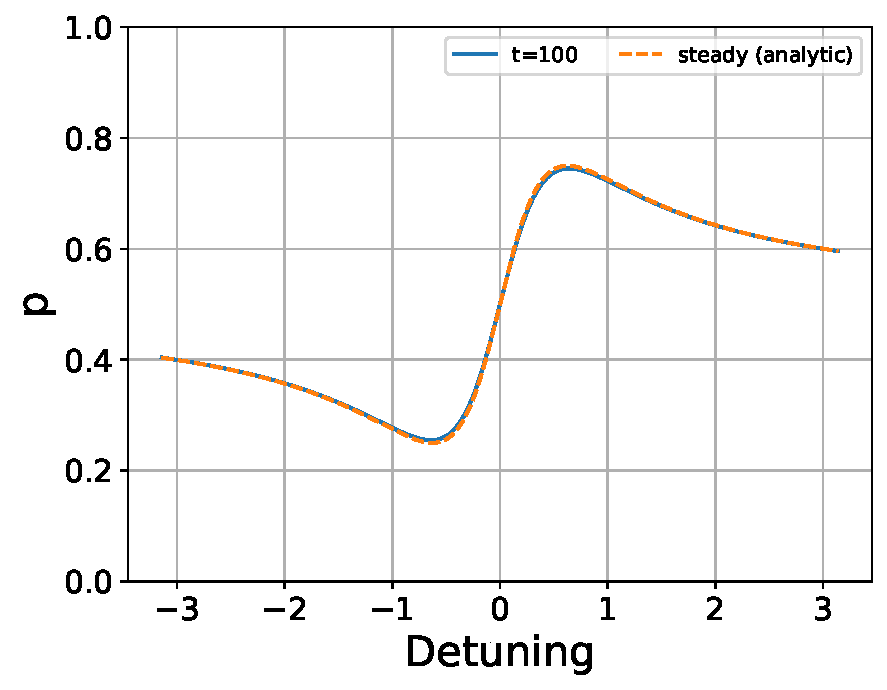
\includegraphics[width=8cm]{../../euriqa/calculations/master_equation/imgs/coherent-scatter_det_theory.pdf}
  \caption{Comparison between the analytic steady state population of $|1\rangle$
    and numerical result from master equation simulation.}
  \label{fig:compare-steady}
\end{figure}

We can compare this with the numerical simulation
result~(Fig.~\ref{fig:compare-steady}) showing very good agreement.\\

\section{Qualitative discussion based on EIT}
From the previous calculation, we can see that the density matrix in the $z$ basis
has non-diagonal terms meaning that there is actually coherence
between the $|0\rangle$ and $|1\rangle$ states.
This agrees with the observation that the selection of scattering state
being important in causing the asymmetry.\\

We also see, as we expected, that when $\delta=0$ the steady state density matrix
represents a pure state $|\psi_d\rangle=\dfrac{|0\rangle-|1\rangle}{\sqrt2}$
which is the EIT dark state. For $\delta\neq0$,
the steady state is not the dark state but it remains fairly closed to the dark state
for small detuning where the asymmetry is the most pronounced.
This suggests that the dark state (and the eigen basis for scattering)
is likely a better starting point / basis to understand the scattering process
and potentially the asymmetry.\\


We'll start by looking at the unitary evolution of the dark state $|\psi_d\rangle$
and see if there's any asymmetry when $\delta$ changes sign.\\

If the initial state of the system is the dark state $|\psi_d\rangle$,
the time derivative of the wavefunction is,
\eqar{
  \begin{split}
    \diff{|\psi\rangle}{t}=&-\ui H|\psi_d\rangle\\
    =&-\frac{\ui}2\paren{\delta\sigma_z+\Omega\sigma_x}\dfrac{|0\rangle-|1\rangle}{\sqrt2}\\
    =&-\frac{\ui}{2\sqrt2}\paren{\paren{\delta-\Omega}|0\rangle+\paren{\delta+\Omega}|1\rangle}
  \end{split}
}
While I'm not sure how it affects the dynamic yet, this indeed shows some asymmetry
between $|0\rangle$ and $|1\rangle$ depending on if $\delta$ and $\Omega$
have the same sign or not. The amplitude of the derivative on $|1\rangle$ is larger
than that on $|0\rangle$ if the two have the same sign,
and smaller if the signs are different.\\

The change in the amplitude of both the $|0\rangle$ and the $|1\rangle$ states
are out-of-phase with their original amplitude so there isn't any first order change
in the state probabilities at $t=0$. We can calculate the second order change
to the wavefunction,
\eqar{
  \begin{split}
    \diff[2]{|\psi\rangle}{t}=&-H^2|\psi_d\rangle\\
    =&-\frac{1}{4}\paren{\delta\sigma_z+\Omega\sigma_x}^2\dfrac{|0\rangle-|1\rangle}{\sqrt2}\\
    =&-\frac{1}{4\sqrt2}\paren{\delta^2+\Omega^2}\paren{|0\rangle-|1\rangle}\\
  \end{split}
}
And from this the second order change to the $|0\rangle$ probability,
\eqar{
  \begin{split}
    \diff[2]{\abs{\langle0|\psi\rangle}^2}{t}=&\diff{}{t}\paren{\langle0|\psi\rangle\diff{\langle\psi|0\rangle}{t}+\diff{\langle0|\psi\rangle}{t}\langle\psi|0\rangle}\\
    =&\langle0|\psi\rangle\diff[2]{\langle\psi|0\rangle}{t}
       +\diff[2]{\langle0|\psi\rangle}{t}\langle\psi|0\rangle
       +2\diff{\langle0|\psi\rangle}{t}\diff{\langle\psi|0\rangle}{t}\\
    =&\frac{1}{4}\paren{\delta-\Omega}^2-\frac{1}{4}\paren{\delta^2+\Omega^2}\\
    =&\frac{\delta\Omega}{2}
  \end{split}
}
i.e. depending on the sign of $\delta\Omega$ the time evolution of the dark state
will put more or less population in the $|0\rangle$ state.
Indeed, we can see this clearly if we simply look at the time evolution
on the Bloch sphere~(Fig.~\ref{fig:darkstate-rotation}).
The initial vector is at $-\hat x$ (blue arrow).
The hamiltonian corresponds to a rotation around the vector
$\delta\hat x+\Omega\hat z$ (red dotted arrow).
Depending on the sign of $\delta$ (actually $\delta\Omega$),
the rotation axis (and therefore the time evolution of the state
shown by the blue dashed circle) may be either above or below the equator.\\

\begin{figure}
  \centering
  \begin{tikzpicture}[scale=1.6]
    \def\R{2.5} % sphere radius
    \def\angEl{20} % elevation angle
    \def\angX{110} % X axis angle
    \filldraw[ball color=white] (0,0) circle (\R);
    \DrawFromCenterText[r=1, center={(3.2, -2.3)}, theta=90, style={->}][above]{$z$}
    \DrawFromCenterText[r=1, center={(3.2, -2.3)}, theta=180, style={->}][left]{$y$}
    \DrawFromCenterText[r=1.5, center={(3.2, -2.3)}, theta=0, phi=\angX, style={->}][above left]{$x$}

    \def\angRot{13} % Rotation axis angle

    \DrawFromCenter[r={-\R * 1.9}, phi={\angX-180}, theta={-\angRot},
    style={red!80!white, line width=2.1, dotted}]
    \node at ({\R * cos(\angRot) * cos(\angX)},
    {\R * (sin(\angRot) + cos(\angRot) * sin(\angX) * sin(\angEl))})
    [red!70!white, circle,fill,inner sep=2.7pt] {};

    \foreach \t in {-60,-30,...,60} {\DrawLatitudeCircle[\R]{\t}}
    \foreach \t in {0,-60,...,-120} {\DrawLongitudeCircle[\R]{\t}}

    \draw[domain=-160:20,smooth,variable=\t,blue,line width=2.1,dashed,>=stealth]
    plot ({\R * (sin(\angRot) * cos(\t) -
      (cos(\angRot)^2+sin(\angRot)^2 * sin(\t)) * cos(\angX))},
    {\R * (sin(\angRot) * cos(\angRot) * (sin(\t) - 1) -
      (cos(\angRot)^2+sin(\angRot)^2 * sin(\t)) * sin(\angX) * sin(\angEl))});

    \DrawFromCenter[r={\R * 1.9}, phi={\angX-180}, theta={-\angRot},
    style={->, >=stealth, red, line width=2.1, dotted}]

    \node at ({-\R * cos(\angRot) * cos(\angX)},
    {\R * (-sin(\angRot) - cos(\angRot) * sin(\angX) * sin(\angEl))})
    [red, circle,fill,inner sep=3pt] {};

    \DrawFromCenter[r=\R, phi={\angX-180}, style={->, blue, line width=1mm}]

    \draw[->,domain=20:200,smooth,variable=\t,blue,line width=2.1,dashed,>=stealth]
    plot ({\R * (sin(\angRot) * cos(\t) -
      (cos(\angRot)^2+sin(\angRot)^2 * sin(\t)) * cos(\angX))},
    {\R * (sin(\angRot) * cos(\angRot) * (sin(\t) - 1) -
      (cos(\angRot)^2+sin(\angRot)^2 * sin(\t)) * sin(\angX) * sin(\angEl))});
  \end{tikzpicture}
  \caption{Unitary evolution of the dark state on the Bloch sphere.
    The blue arrow represent the dark state $|\psi_d\rangle$
    and the red dotted arrow is the rotation axis determined by the Hamiltonian.
    The blue dashed circle is the trajectory the state make on the Bloch sphere.}
  \label{fig:darkstate-rotation}
\end{figure}

Based on these observation, here is a semi-quatitative explaination of this phenomena.
\begin{enumerate}
\item The scattering process preferentially pumps the system into the dark state
  $\dfrac{|0\rangle-|1\rangle}{\sqrt2}$.
\item The Hamiltonian rotates the system around the axis $\delta\hat x+\Omega\hat z$
  on the Bloch sphere, which is out of the equator plane when $\delta\neq0$.
\item The interaction between these two effects means that the system
  is being pumped towards one side of the rotation axis
  and since the rotation axis is tilted the resulting state will have an uneven
  distribution between the $|0\rangle$ and $|1\rangle$ states.
\end{enumerate}
In short, the symmetry in $x$ is broken by the scattering/optical pumping term
and this asymmetry is projected onto $z$ by the Hamiltonian.\\

This can also explain the rough shape of the asymmetry. As $\delta$ increases,
the coupling between $x$ and $z$ increases and there's more asymmetry
in the steady state population. The coupling maximizes when $\delta=\Omega$
(i.e. $45^\circ$ tilted axis) after which point the steady state population
asymmetry decreases again.\\

We could also extend this explaination to other system configurations as well.
If somehow the initial state of the scattering is random but the final state
is always $\dfrac{|0\rangle+|1\rangle}{\sqrt2}$, this would result in an optical
pumping effects towards $+x$ direction which would produce an asymmetry
in the population in the other direction (confirmed by simulation).
Similarly, if the OP process (either because of the initial or final state)
is along the $y$ axis, there will be no asymmetry based on the detuning
since it is orthogonal to the rotation axis.
There will, however, still be an asymmetry in the population
since the rotation caused by the Hamiltonian will move the dark state
closed to one of the poles.

\end{document}
